\documentclass[../../main.tex]{subfiles}
\begin{document}

{\bf [解答]}

与えられた関数
\begin{align}
  f(x) = x^2 + ax + b \quad (0 \le x \le 1) \label{eq:1}
\end{align}
について考える．$[0,1]$での最小値$m$は，$f(x)$の軸の位置$x=\dfrac{-a}{2}$で場合分けすると以下のようになる．

\begin{enumerate}
  \item[ア] $-\dfrac{a}{2} \le 0 \iff a \ge 0$ の時, $m = f(0) = b$
  \item[イ] $0 \le -\dfrac{a}{2} \le 1 \iff -2 \le a \le 0$ の時, $m = f\left(-\dfrac{a}{2}\right) = -\dfrac{1}{4}a^2 + b$
  \item[ウ] $1 \le -\dfrac{a}{2} \iff a \le -2$ の時, $m = f(1) = a + b + 1$
\end{enumerate}

\begin{figure}[htb]
  \centering
  \begin{tikzpicture}[scale=1.05, >=stealth, every node/.style={font=\small}]
    % --------------------------------------------------------
    % (ア) 軸が区間の左側: -a/2 <= 0
    % --------------------------------------------------------
    \begin{scope}[shift={(0, 0)}]
      \draw[->, thick, gray!80!black] (-0.8, 0) -- (1.8, 0) node[right] {$x$};
      \draw[->, thick, gray!80!black] (0, -0.3) -- (0, 2.3) node[above] {$y$};
      \node[below left=2pt] at (0, 0) {$O$};
      \node[below] at (1, 0) {$1$};
      \draw[gray!50, dotted] (1, 0) -- (1, 2.0);

      % 軸 x = -0.4
      \draw[teal!75!black, dashed] (-0.4, -0.2) -- (-0.4, 2.0);
      \node[below, teal!75!black, font=\footnotesize] at (-0.4, -0.2) {$-\frac{a}{2}$};

      % 放物線: f(x) = 1.2*(x+0.4)^2 + 0.3
      \draw[blue!40, dashed, domain=-0.7:0, samples=30] plot (\x, {1.2*(\x+0.4)*(\x+0.4) + 0.3});
      \draw[line width=1.4pt, blue!85!black, domain=0:1, samples=40] plot (\x, {1.2*(\x+0.4)*(\x+0.4) + 0.3});
      \draw[blue!40, dashed, domain=1:1.3, samples=20] plot (\x, {1.2*(\x+0.4)*(\x+0.4) + 0.3});

      % 最小点 x = 0
      \node[circle, fill=red!85!black, inner sep=1.4pt] at (0, 0.492) {};
      \node[left=2pt, red!85!black, font=\footnotesize] at (0, 0.65) {$m=f(0)$};

      \node[below=18pt, font=\small] at (0.5, 0) {ア: $-\frac{a}{2} \le 0$};
    \end{scope}

    % --------------------------------------------------------
    % (イ) 軸が区間内: 0 <= -a/2 <= 1
    % --------------------------------------------------------
    \begin{scope}[shift={(3.8, 0)}]
      \draw[->, thick, gray!80!black] (-0.5, 0) -- (1.8, 0) node[right] {$x$};
      \draw[->, thick, gray!80!black] (0, -0.3) -- (0, 2.3) node[above] {$y$};
      \node[below left=2pt] at (0, 0) {$O$};
      \node[below] at (1, 0) {$1$};
      \draw[gray!50, dotted] (1, 0) -- (1, 1.8);

      % 軸 x = 0.5
      \draw[teal!75!black, dashed] (0.5, -0.2) -- (0.5, 2.0);
      \node[below, teal!75!black, font=\footnotesize] at (0.5, -0.2) {$-\frac{a}{2}$};

      % 放物線: f(x) = 2.0*(x-0.5)^2 + 0.3
      \draw[blue!40, dashed, domain=-0.3:0, samples=20] plot (\x, {2.0*(\x-0.5)*(\x-0.5) + 0.3});
      \draw[line width=1.4pt, blue!85!black, domain=0:1, samples=40] plot (\x, {2.0*(\x-0.5)*(\x-0.5) + 0.3});
      \draw[blue!40, dashed, domain=1:1.3, samples=20] plot (\x, {2.0*(\x-0.5)*(\x-0.5) + 0.3});

      % 最小点 x = 0.5 (頂点)
      \node[circle, fill=red!85!black, inner sep=1.4pt] at (0.5, 0.3) {};
      \node[above=2pt, red!85!black, font=\footnotesize] at (0.5, 0.3) {$m=f(-\frac{a}{2})$};

      \node[below=18pt, font=\small] at (0.5, 0) {イ: $0 \le -\frac{a}{2} \le 1$};
    \end{scope}

    % --------------------------------------------------------
    % (ウ) 軸が区間の右側: 1 <= -a/2
    % --------------------------------------------------------
    \begin{scope}[shift={(7.6, 0)}]
      \draw[->, thick, gray!80!black] (-0.5, 0) -- (2.1, 0) node[right] {$x$};
      \draw[->, thick, gray!80!black] (0, -0.3) -- (0, 2.3) node[above] {$y$};
      \node[below left=2pt] at (0, 0) {$O$};
      \node[below] at (1, 0) {$1$};
      \draw[gray!50, dotted] (1, 0) -- (1, 1.8);

      % 軸 x = 1.4
      \draw[teal!75!black, dashed] (1.4, -0.2) -- (1.4, 2.0);
      \node[below, teal!75!black, font=\footnotesize] at (1.4, -0.2) {$-\frac{a}{2}$};

      % 放物線: f(x) = 1.2*(x-1.4)^2 + 0.3
      \draw[blue!40, dashed, domain=-0.2:0, samples=20] plot (\x, {1.2*(\x-1.4)*(\x-1.4) + 0.3});
      \draw[line width=1.4pt, blue!85!black, domain=0:1, samples=40] plot (\x, {1.2*(\x-1.4)*(\x-1.4) + 0.3});
      \draw[blue!40, dashed, domain=1:1.7, samples=30] plot (\x, {1.2*(\x-1.4)*(\x-1.4) + 0.3});

      % 最小点 x = 1
      \node[circle, fill=red!85!black, inner sep=1.4pt] at (1, 0.492) {};
      \node[right=2pt, red!85!black, font=\footnotesize] at (1, 0.65) {$m=f(1)$};

      \node[below=18pt, font=\small] at (0.5, 0) {ウ: $1 \le -\frac{a}{2}$};
    \end{scope}
  \end{tikzpicture}
  \caption{軸 $x = -\dfrac{a}{2}$ の位置による $f(x)$ の最小値の場合分け．}
  \label{fig:1971_3_axis_cases}
\end{figure}

次に，$a+2b \le 2$を満たす $(a, b)$ の存在領域は下図斜線部 (境界含む) である.

\begin{figure}[htb]
  \centering
  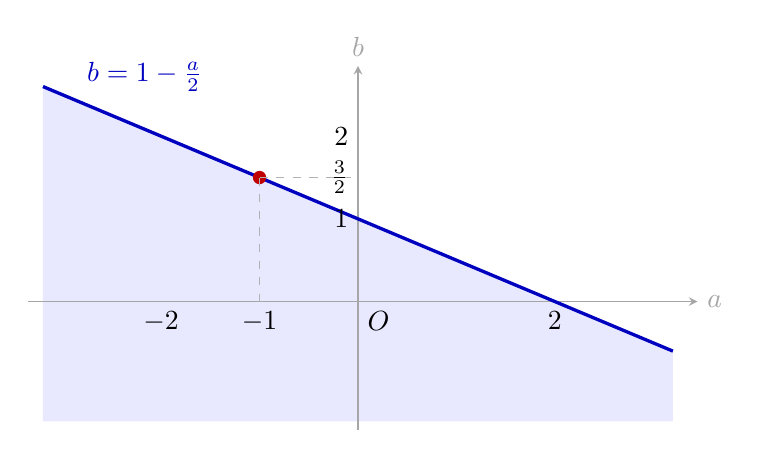
\begin{tikzpicture}[x=1.25cm, y=1.05cm, >=stealth,
      axis/.style={gray!70, thin},
    boundary/.style={blue!75!black, very thick}]
    \coordinate (O) at (0,0);
    \coordinate (Peak) at (-1,1.5);
    \fill[blue!9] (-3.2,2.6) -- (3.2,-0.6) --
    (3.2,-1.45) -- (-3.2,-1.45) -- cycle;
    \draw[axis, ->] (-3.35,0) -- (3.45,0) node[right] {$a$};
    \draw[axis, ->] (0,-1.55) -- (0,2.85) node[above] {$b$};
    \draw[boundary] (-3.2,2.6) -- (3.2,-0.6);
    \node[circle, fill=red!75!black, inner sep=1.7pt] at (Peak) {};
    \draw[gray!60, dashed] (Peak) -- (-1,0);
    \draw[gray!60, dashed] (Peak) -- (0,1.5);
    \node[below right] at (O) {$O$};
    \node[below] at (-2,0) {$-2$};
    \node[below] at (-1,0) {$-1$};
    \node[below] at (2,0) {$2$};
    \node[left] at (0,1) {$1$};
    \node[left] at (0,1.5) {$\frac{3}{2}$};
    \node[left] at (0,2) {$2$};
    \node[blue!75!black, above right] at (-2.85,2.425) {$b=1-\frac{a}{2}$};
  \end{tikzpicture}
  \caption{ $(a,b)$ の領域（青色）と，最大値を与える点 $(-1,\dfrac{3}{2})$．}
  \label{fig:1971_3_parameter_region}
\end{figure}

よって，それぞれの場合での$m$の最大値は以下のようになる．

\subparagraph{ア: $0 \le a$の時}

この時は$m=b$より，$b=1$つまり$a=0$の時に最大値
\begin{align}
  \max m = 1 \quad (a,b)=(0,1)
\end{align}
をとる．

\subparagraph{イ: $-2 \le a \le 0$の時}

この時は$m=\dfrac{-1}{4}a^2+b$より，まず$a$を固定して$b$を動かすと$m$は$b$について単調増加だから
\begin{align}
  m \le -\dfrac{1}{4}a^2 - \dfrac{1}{2}a + 1 = -\dfrac{1}{4}(a+1)^2 + \dfrac{5}{4}
\end{align}
であり，次に$a$を動かすとこれは$a=-1$つまり$b=\dfrac{3}{2}$の時に最大値
\begin{align}
  \max m = \dfrac{5}{4} \quad (a,b) = (-1,3/2)
\end{align}
を取る．

\subparagraph{ウ: $a \le -2$の時}

この時は$m=a+b+1$より，まず$a$を固定して$m$を動かすと$m$は$b$について単調増加だから
\begin{align}
  m \le a + 1 - \dfrac{1}{2}a + 1 = \dfrac{1}{2}a + 2
\end{align}
である．次に$a$を動かすとこれは$a=-2$つまり$b=2$の時に最大値
\begin{align}
  \max m = 1 \quad (a,b) = (-2,2)
\end{align}
をとる．
\casesend

以上から $(a, b) = \left(-1, \dfrac{3}{2}\right)$ が $m$ を最大にする.

\newpage

\end{document}
